\section{Elongation} %do these last!
After escaping the \gls{pic}, \gls{pol2} enters the phase of productive elongation.
During this phase, the polymerase travels along DNA, catalysing the addition of nucleotides to the growing RNA molecule that is being synthesised.
The simple synthesis of the RNA, however, is not enough to qualify a mature transcript.
Several essential processing steps take place during transcription elongation and contribute to the production of fully formed transcripts.
Among these, the addition of the 5' cap, addition of a poly(A) tail, and formation of an export-competent transcript all rely on the presence of \gls{pol2} and the \gls{tec} in order to be carried out properly.
The precise composition of the \gls{tec} is poorly understood. 
However, as \gls{pol2} progresses through the transcription unit, several complexes and co-factors are known to dynamically associate with it in order to enact the various maturation steps.  
Transcription elongation is therefore a highly regulated activity that coordinates several different processes to produce mature transcripts.
This regulation is enacted by the cell through several distinct mechanisms, such as the phosphorylation of the \gls{ctd} and the modification of histones.
These very same regulation mechanisms---along with important regulatory sequences---will eventually mark the end of transcription elongation and the transition to transcription termination.

\subsection{Elongation through chromatin}
Chromatin represents an extremely repressive barrier to any kind of DNA based process.
As I briefly touched upon in previous sections, chromatin components---histones---need to be actively dislodged from promoter regions in order to allow the \acrlong{pic} to assemble.
Elongating \gls{pol2} faces very similar problems, as in order to synthesise the RNA, it has to move through an array of nucleosomes without losing contact with DNA.
Although \invitro{} evidence has shown that \gls{pol2} can effectively elongate through a single nucleosome \citep{lorch:1987:nucleosomes}---possibly due to spontaneous disassembly and reassembly of nucleosomes, a process that was recently shown to happen every few seconds\citep{kim:2016:singlemolecule}---the elongation complex alone is not enough to mediate transcription through multiple nucleosomes.

\begin{figure}[ht]

\centering
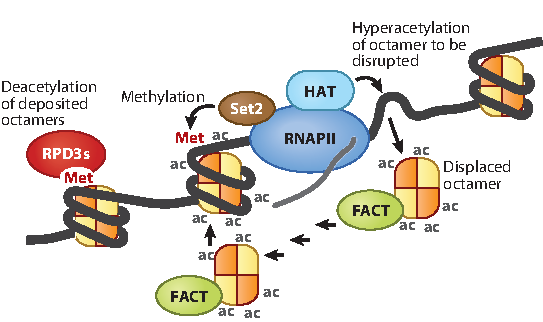
\includegraphics[width=\textwidth]{figures/introduction/nucTranscription}
\caption[Mechanism of transcription through chromatin.]{Overview of the main actors in the mechanism of transcription through chromatin.
Nucleosomes are destabilized through acetylation and chaperoned away---either partially or completely---by \gls{fact} and other complexes.
Addition of methyl groups to histone tails allows the recruitment of \gls{hdacs} and the restoration of chromatin structure.
adapted from \citep{selth:2010:transcript}. }
\label{fig:nucTranscription}

\end{figure}

The \gls{tec} can overcome this problem by enlisting the help of several histone chaperones and chromatin remodeling complexes, as well as by exploiting post translational modifications of histones (Fig: \ref{fig:nucTranscription}). 
The current model for transcription through nucleosomes posits that, depending on the intensity of transcription, histones can either be completely removed from DNA, or be partially destabilized as to allow \gls{pol2} to more easily transcribe through them \citep{kulaeva:2013:mechanism}.
The most notable actors in this phase are \gls{hats} such as Gcn5 and the \gls{fact} (\glsdesc{fact}) complex \citep[for review see:][]{reinberg:2006:de}. 
\gls{hats} are posited to travel with the polymerase, depositing an acetyl group on histone tails.
This has the consequence of destabilizing inter-nucleosome interactions as well as lowering the affinity for DNA by increasing the negative charge, resulting in a more relaxed chromatin structure and more unstable nucleosomes.
Once histones are acetylated, \gls{fact}---also travelling with the polymerase---destabilizes the H2A-H2B dimer \footnote{
Two of the four core components of a histone. Histones are composed of two H2A-H2B dimers and one H3-H4 tetramer arranged in a symmetrical structure. 
}, removing it and facilitating transcription through the remaining incomplete nucleosome structure. 

We saw how, in order to efficiently elongate, \gls{pol2} needs to destabilize the chromatin structure.
However, this destabilization results in a more relaxed structure that can potentially give rise to intragenic transcription initiation.
In order to prevent this phenomenon, the composition, modifications, and overall structure of nucleosomes must be reset after the passage of \gls{pol2}. 
Specific histone chaperones such as Spt6, together with methil-transferases and \gls{hdacs}, are involved in this process.
First, Spt6 and other histone chaperones reconstruct a complete histone in the wake of transcribing \gls{pol2}.
Subsequently, methil-transferases such as Set2 methilate lysine 36 on histone H3. 
Although this modification---unlike acetylation---has no structural consequences on the organization of nucleosomes, it can act as a platform for recruitment of \gls{hdacs}.
The RPD3 complex has high affinity for H3K36 methilation and is recruited immediately after the passage of \gls{pol2} in order to remove the acetyl groups from histones and thus reset the structure of chromatin.

\subsection{Transcriptional pausing} \label{pausing}
Nucleosomes do not represent the only obstacle to productive elongation.
A number of occurrences can prevent \gls{pol2} from elongating forward, such as DNA damage, misincorporation of a nucleotide, or collision with another DNA-bound protein.
While the cell has evolved complex---and often slow---mechanisms to deal with the more extreme instances \footnote{For example when DNA is damaged,the cell employs ubiquitinylation and degradation of the largest subunit of \gls{pol2} to resolve pausing.}, transcriptional pausing represents the first and common consequence to all the above-cited events. 
Because reversible pause-inducing events are relatively common during transcription---pausing has been documented in front of every nucleosome \citep{churchman:2011:nascent}---the cell evolved an all-purpose mechanism called backtracking.
The purpose of backtracking is to quickly resolve pausing before the slower, more complex systems are called into action. 

During backtracking---being unable to translocate forward---\gls{pol2} moves backwards, retracing its steps anywhere form 4-5 up to 12-15 nucleotides \citep{cheung:2011:structural}.
This backwards movement causes part of the already synthesized RNA to slide forward into a channel connected to the outside of the complex.
Presence of RNA into the channel promotes the binding of TFIIS \footnote{Also known as \emph{Dst1}} to the complex \citep{cheung:2011:structural}.
This stimulates the intrinsic endonucleolytic activity of \gls{pol2}, which results in cleavage of the extruding RNA and realignment of the 3' end of the nascent transcript with the catalytic site of the polymerase.
At this point, \gls{pol2} has effectively reset its position, having moved back and gotten rid of the extra segment of RNA. 
It can therefore restart its forward translocation and resume the normal catalytic activity.

While this mechanism is a very effective way of dealing with minor pausing events and nucleotide misincorporations, it is not enough to deal with more stubborn pausing agents.
Notably, it has been recently shown that presence of the transcription factor Reb1 on DNA is sufficient to pause the elongation of \gls{pol2} in a way that is unaffected by backtracking; ultimately resulting in the disassembly of the elongation complex and release of the transcript \cite{colin:2014:roadblock}.
 


\subsection{The CTD}
\gls{pol2} and the elongation complex are fundamental elements in coordinating many of the co-transcriptional processes that contribute to the maturation of the nascent RNA.
In order to dynamically recruit all the necessary factors and complexes in a timely fashion, the largest subunit of \gls{pol2} has evolved an unstructured C-terminal domain composed, in \cer, of 26 repeats of the heptapeptide \ctdshort{} \footnote{\ctdlong{} in expanded nomenclature}.
This cluster of repeats can be differentially phosphorylated in different phases of transcription elongation, acting as a dynamically changing interaction surface for different co-factors. 

\subsubsection{CTD phosphorylation dynamics} 
The \gls{ctd} heptapeptide contains a high number of phosphorylatable residues.
Out of the 7 amminoacids, 5 can support the addition of a phosphate group: \tyr{}, \sert{}, \thr{}, \serf{}, and \sers{}.
The combinatorial phosphorylation of \sert{} and \serf{}, however, provides the majority of the functional contribution to transcription elongation and it was recently shown that phospho-groups at these two residues are more abundant than on any of the other residues \citep{suh:2016:direct}. Unlike \sert{} and \serf{}, understanding of the consequences of \tyr{}, \thr{}, and \sers{} phosphorylation is still limited. 
Modification of \thr{} and \sers{} has specialized roles in the transcription of particular species\footnote{In vertebrates, \thr{} has been shown to be important in the processing---but not transcription---of histone genes \cite{hsin:2011:rnap}, while \sers{} was shown to recruit the \gls{ctd} phosphatase Rpap2 specifically to \gls{sns} genes \citep{egloff:2012:role}.}, while the modification of \tyr{} has no attributed roles as of yet. 
In light of this, in the following paragraphs I will focus mainly on the mechanisms and effects of \sert{} and \serf{} phosphorylation.

\begin{figure}[ht]

\centering
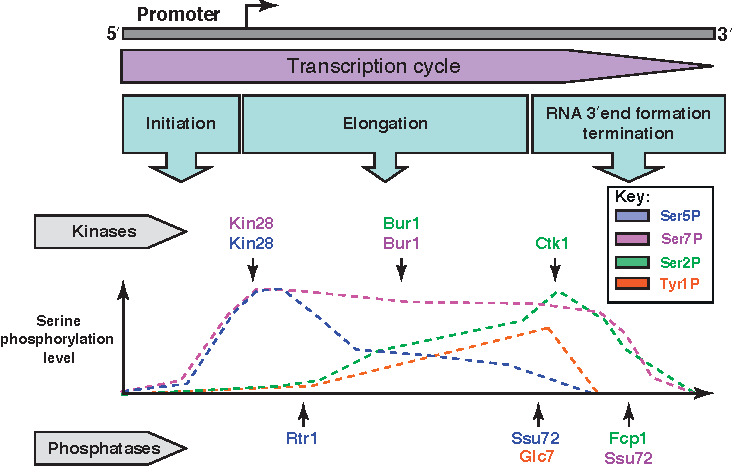
\includegraphics[width=\textwidth]{figures/introduction/ctdPhospho}
\caption[CTD phosphorylation states throughout the transcription cycle.]{
General view of \sert{}, \serf{}, and \sers{} phosphorylation along the transcription cycle,
kinases and phosphatases involved in \gls{ctd} modification are represented immediately above and below the graph.
The two main phosphorylation states, \sert{} and \serf{}, are dominant at the 3' and 5' respectively, reflecting their functional roles in the termination and early elongation phases of transcription.
\sers{} is consistently present throughtout the transcription cycle, but its functional impact in yeast remains elusive. Adapted from \citep{egloff:2012:updating}.
}
\label{fig:ctdPhospho}

\end{figure}

During the Initiation phase of transcription, the \gls{ctd} of \gls{pol2} starts off unphosphorylated (see Fig: \ref{fig:ctdPhospho}).
When the \gls{pic} is fully assembled, Kin28, a catalytic subunit of the general transcription factor TFIIH, phosphorylates the CTD heptapeptide on \serf{}.
In \cer{}, the \gls{ctd} remains mostly \serf{} phosphorylated for the first 450 nucleotides of transcription elongation \citep{mayer:2010:uniform}. 
After this point the combined action of the \serf{}-phosphatase Rtr1 \citep{mosley:2009:rtr1, hunter:2016:phosphatase} and the \sert{}-kinases Bur1 and Ctk1 \citep{qiu:2009:phosphorylation} make \sert{} the most prominent mark \footnote{
It is interesting to note that the phosphorylation state of \gls{pol2} \gls{ctd} is independent of transcript length, but exclusively depends on the amount of nucleotides from the \gls{tss}. 
This will have important implications for the termination of non-coding transcripts.}.
Despite phosphorylation of \sert{} reaching saturation about 600 nucleotides from the \gls{tss} \citep{mayer:2010:uniform}, \serf{} phosphorylation is still present on many repeats, resulting in the presence of a double phosphorylation pattern with important functional consequences (see below).
Only Towards the 3' end of the gene the action of \gls{ctd} phosphatase Ssu72 completely abrogates the \serf{}-P mark, leaving \sert{}-P as the only active mark.
Finally, additional activity of the Fcp1 phosphatase results in the removal of most phospho-marks from the \gls{ctd}, readying the polymerase for another round of transcription.

%Recent studies tried to explore the differences between distal and proximal \gls{ctd} repeats, 
\subsubsection{Functional interactions}

As I outlined above, the transcription cycle follows specific patterns of \gls{ctd} phosphorylation: unphosphorylated \gls{ctd} is recruited to promoter regions, \serf{}-P dominates during early elongation and gradually makes way for \sert{}-P, which is the dominant mark in the later stages of transcription. Each of these stages comes with the potential to interact with numerous co-factors and provides modularity to the elongation complex.

The unphosphorylated state of free-form \gls{pol2} \gls{ctd} allows the polymerase to interact with the mediator complex; an interaction that is thought to contribute to the recruitment of \gls{pol2} to active promoters. 
Once the \gls{pic} is assembled, the polymerase needs to escape the promoter and leave the \acrlong{pic} behind.
The modifications that take place at this stage, namely \serf{} phosphorylation, are thought to disrupt the interaction between \gls{pol2} and mediator---thereby allowing promoter clearance---although evidence remains inconclusive \citep{so:2007:hyperphosphorylation, davis:2002:structure}.

The presence of \serf{} mark during early elongation has two direct consequences: it stimulates capping of the nascent transcript through recruitment of the capping enzymes, and it has the potential to promote early transcription termination through the recruitment of the \gls{nns} complex.
While capping is ubiquitous and required to prevent premature degradation of the transcript, early termination is a quality control mechanism that requires (in addition to \serf{}-P) the presence of specific sequence elements on the nascent transcript and will be described in detail in a future section.

Studies in mammals have reported that the \gls{ctd} is required for splicing to occur properly, in particular heptapeptides containing both \serf{} and \sert{} phopshorylation are known to recruit several splicing factors. Recent studies in \cer{}, however, show differential phosphorylation patterns in intronless and intron-containing genes, hinting at a possible splicing role for \gls{ctd} phopshorylation in yeast \cite{milligan:2016:strandspecific}.

Towards the end of the transcription cycle, \sert{}-P becomes the most prominent mark. 
This phase sees the recruitment of a number of different actors.
Chromatin remodelers and histone modifying complexes such as Set2 and Spt6 are recruited through the \gls{ctd}, making sure that the structure of nucleosomes is maintained.

Finally, 3' end processing, termination, and export are all affected by the \gls{ctd}. binding of components of the cleavage and polyadenylation complex such as Pcf11 and Rtt103 stimulates the termination of transcription and the processing of the transcript 3' end (such as poly(A) tail addition), while recruitment of export factors such as Yra1 direct a rapid and efficient export to the cytoplasm.
 


\clearpage